\documentclass{standalone}
\usepackage{tikz}
\usepackage{ctex,siunitx}
\usepackage{tkz-euclide}
\usepackage{amsmath}
\usetikzlibrary{patterns, calc}
\usetikzlibrary {decorations.pathmorphing, decorations.pathreplacing, decorations.shapes,}
\begin{document}
\small
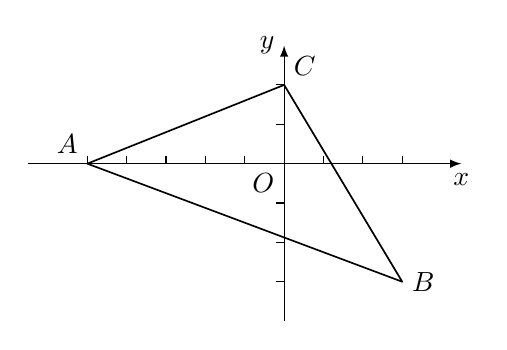
\begin{tikzpicture}[>=latex,scale=0.5]
  \draw[thin,->](-6.5,0)--(4.5,0)node[below]{$x$};
  \draw[thin,->](0,-4)--(0,3)node[left]{$y$};
  \tkzDefPoints{0/0/O,-5/0/A,3/-3/B,0/2/C}
  \foreach \x in {-5,...,3}
  {
    \draw[thin](\x,0)--++(0,0.2);
  }
  \foreach \x in {-3,...,2}
  {
    \draw[thin](0,\x)--++(-0.2,0);
  }
  \tkzDrawPolygon[semithick](A,B,C)
  \tkzLabelPoints[above left](A)
  \tkzLabelPoints[above right](C)
  \tkzLabelPoints[right](B)
  \tkzLabelPoints[below left](O)
  % \draw(-0.5,0)arc(0:30:0.5)node[midway,right]{$\alpha$};
\end{tikzpicture}
\end{document}